\documentclass{article}

\usepackage{fullpage}
\usepackage{url}
\usepackage{bbm}
\usepackage{graphicx}
\usepackage{amsmath}
\usepackage{physics}
\usepackage{mathtools}
\usepackage{bbold}
\usepackage{slashed}
\usepackage{pxfonts}
\usepackage{multicol}
\usepackage{mathptmx}
\usepackage{simplewick}
\usepackage{placeins}

\usepackage{lmodern}
\usepackage[T1]{fontenc}
\usepackage[fontsize=13.5pt]{fontsize}

\DeclareMathOperator{\erfi}{erfi}
\newcommand{\R}{\ensuremath{\mathbb{R}}}
\newcommand{\C}{\ensuremath{\mathbb{C}}}

\title{Quantum Field Theory I Excercise 5}
\author{Idan Stark}
\date{\today}

\begin{document}
\maketitle

\section{The beta function of Yukawa theory}
\subsection{The momentum-space 3-point correlation function}
The momentum space 3-point correlation function $G^{(3)} = \langle \bar{\psi}(p_1)\psi(p_2)\phi(p_3) \rangle$ has a single first order contributing diagrams, which is the treelike single vertex diagram (figure 1). There are techincally an additional tadpole diagram, but as $\langle \phi \rangle = 0$, we can ignore it.
This gives the value (using momentum space Feynman rules for the correlation function):
\begin{equation}
    G^{(3)} = \langle \bar{\psi}(p_1)\psi(p_2)\phi(p_3) \rangle = -ig + \mathcal{O}(g^3)
\end{equation}
The $g^3$ correction has four diagrams:
\begin{itemize}
    \item The 3-point triangle loop diagram
    \item Three loops extensions to the first order
\end{itemize}
These diagrams are diaplyed in figure 2.
\begin{figure}[!htbp]
    \centering
    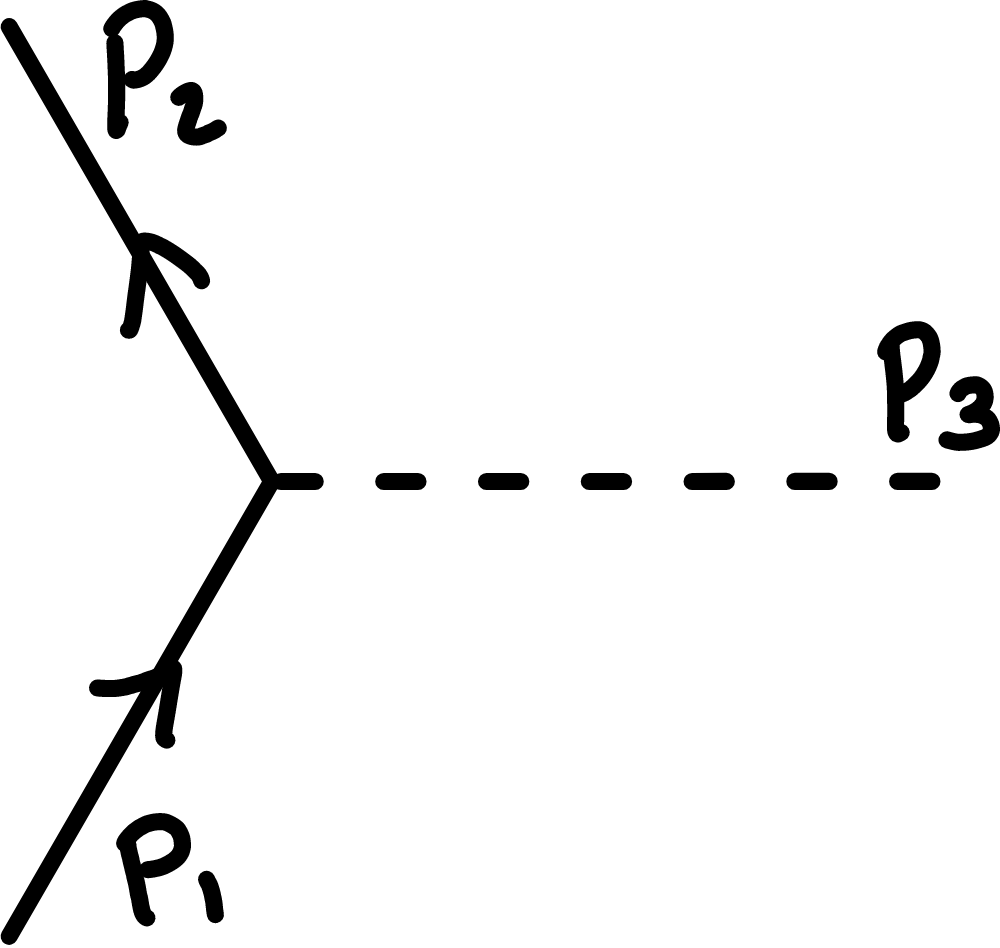
\includegraphics[width=0.5\textwidth]{figures/figure1.png}
    \caption{The treelike single vertex diagram.}
\end{figure}
\begin{figure}[!htbp]
    \centering
    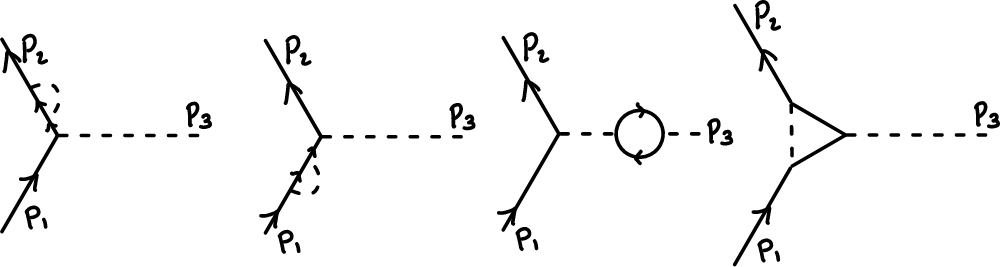
\includegraphics[width=0.8\textwidth]{figures/figure2.png}
    \caption{The four corrections of order $g^3$. The rightmost one is the 3-point triangle loop diagram, while the other three are the loop extensions to the single vertex treelike diagram}
\end{figure}
\subsection{The Callan-Symanzik equation}
Using the renormalization factors
\begin{equation}
    \phi_0 = \sqrt{Z_\phi}\phi
    \qquad
    \psi_0 = \sqrt{Z_\psi}\psi
\end{equation}
We can write the correlation function:
\begin{equation}
    \langle \bar{\psi}_0(p_1)\psi_0(p_2)\phi_0(p_3) \rangle = \sqrt{Z_\phi}Z_\psi G^{(3)}(p_1, p_2, p_3; g(M), M)
\end{equation}
Applying $M \frac{d}{dM}$ will give the Callan-Symanzik equation:
\begin{equation}
    \left[
        \gamma_\phi + 2\gamma_\psi +
        \beta\partial_g + M\partial_M
    \right]G^{(3)} = 0
\end{equation}
Where
\begin{equation}
    \gamma_\phi = \frac{1}{2Z_\phi}M\frac{dZ_\phi}{dM}
    \qquad
    \gamma_\psi = \frac{1}{2}M\frac{dZ_\psi}{dM}
    \qquad
    \beta = M \frac{dg}{dM}
\end{equation}
\subsection{Calculating $\gamma_\phi$}
For high energies $p^2 > m_\phi^2, m_\psi^2$, we can consider the theory as practically massless, and use exactly the same dimensional analysis we used in class:
\begin{equation}
    G^{(2)}_\phi(p) = \frac{i}{p^2} - \frac{i}{p^2}\left(ip^2 \left(A \log\frac{\Lambda^2}{p^2} + C_1\right) + iC_2\Lambda^2\right)\frac{i}{p^2} + \frac{i}{p^2}\left(ip^2\delta_{z_\phi} - i\delta_{m_\phi}\right)\frac{i}{p^2}
\end{equation}
Which means:
\begin{equation}
    \Sigma\left(p^2\right) = p^2 \left(A \log\frac{\Lambda^2}{p^2} + C_1\right) - C_2\Lambda^2 - p^2\delta_{z_\phi} + \delta_{m_\phi}
\end{equation}
And the renormalization condition
\begin{equation}
    \frac{d}{dp^2}\Sigma \Bigg|_{p^2 = M^2} = 0
\end{equation}
Gives:
\begin{equation}
    A \log\frac{\Lambda^2}{M^2} - A + C_1 - \delta_{z_\phi} = 0
\end{equation}
\begin{equation}
    \delta_{z_\phi} = A \log\frac{\Lambda^2}{M^2} - A + C_1
\end{equation}
Therefore, to find $\gamma_\phi$ we can write:
\begin{equation}
    \frac{d\delta_{z_\phi}}{dM} = A\frac{1}{\frac{\Lambda^2}{M^2}}\frac{-2\Lambda^2}{M^3} = \frac{-2A}{M}
\end{equation}
\begin{equation}
    \gamma_\phi = \frac{1}{2}M\frac{d\delta_{z_\phi}}{dM} = -A
\end{equation}
As we saw in the tutorial about Yukawa propegators:
\begin{equation}
    \Sigma(p^2) \supset
    \frac{3g^2}{4\pi^2} \int_0^1 dx \left[
        \left(m_\psi^2 - x(1 - x)p^2\right)
        \log\left(\frac{1}{m_\psi^2 - x(1 - x)p^2}\right)
    \right]
\end{equation}
Which in the high energy limit $m_\psi \ll p$ gives:
\begin{equation}
    \Sigma(p^2) \supset
    - \frac{3g^2}{4\pi^2} \int_0^1 dx 
        x(1 - x)p^2
        \log\left(\frac{1}{p^2}\right) = - \frac{g^2}{8\pi^2}p^2
        \log\left(\frac{1}{p^2}\right)
\end{equation}
And so we get:
\begin{equation}
    \gamma_\phi = \frac{g^2}{8\pi^2}
\end{equation}
\subsection{Calculating $\gamma_\psi$}
We again consider the theory as massless, and write the Fermion propegator as we saw in the same tutorial:
\begin{equation}
    G^{(2)}_\psi (p) = \frac{i}{\slashed{p} - \tilde{\Sigma}(p) + i\epsilon}
\end{equation}
Where
\begin{equation}
\begin{gathered}
    \tilde{\Sigma}(p) \supset -\frac{g^2}{16\pi^2} \int_0^1 dx \left[
        \left(m_\psi + x\slashed{p}\right)\log\frac{1}{- x(1 - x)p^2 + xm_\phi^2 + (1 - x)m_\psi^2}
    \right] \\ \xrightarrow{m_\phi, m_\psi \ll M}
    -\frac{g^2}{16\pi^2} \int_0^1 x dx 
        \slashed{p}\log\frac{1}{p^2} = -\frac{g^2}{32\pi^2}\slashed{p}\log\frac{1}{p^2}
\end{gathered}
\end{equation}
Using again the same logic as in the scalar case, in the massless case we can use dimensional arguments to get a similar propegator up to second order in $g$:
\begin{equation}
    G^{(2)}_\psi(p) = \frac{i}{\slashed{p}} - \frac{i}{\slashed{p}}\left(i\slashed{p} \left(A \log\frac{\Lambda^2}{p^2} + C_1\right) + iC_2\Lambda\right)\frac{i}{\slashed{p}} + \frac{i}{\slashed{p}}\left(i\slashed{p}\delta_{z_\psi} - i\delta_{m_\psi}\right)\frac{i}{\slashed{p}}
\end{equation}
Giving:
\begin{equation}
    \tilde{\Sigma}\left(p\right) = \slashed{p} \left(A \log\frac{\Lambda^2}{p^2} + C_1\right) - C_2\Lambda - \slashed{p}\delta_{z_\psi} + \delta_{m_\psi}
\end{equation}
We can write it as:
\begin{equation}
    \tilde{\Sigma}\left(p\right) = \slashed{p} \tilde{\Sigma}^{(0)}(p^2) + \tilde{\Sigma}^{(1)}(p^2)
\end{equation}
Where
\begin{equation}
    \tilde{\Sigma}^{(0)}(p^2) = \left(A \log\frac{\Lambda^2}{p^2} + C_1\right) - \delta_{z_\psi}
    \qquad
    \tilde{\Sigma}^{(1)}(p^2) = -C_2\Lambda + \delta_{m_\psi}
\end{equation}
Using the second renormalization condition:
\begin{equation}
    \tilde{\Sigma}^{(0)}(M^2) = 0
\end{equation}
Gives:
\begin{equation}
    \delta_{z_\psi} = A \log\frac{\Lambda^2}{M^2} + C_1
\end{equation}
This will again give:
\begin{equation}
    \gamma_\psi = \frac{1}{2}M d\frac{\delta_{z_\psi}}{dM} = - A = \frac{g^2}{32\pi^2}
\end{equation}
\subsection{Finiding the $\beta$ function}
The 1-loop correction to the 3 point function is a result of the four diagrams we saw above. Each diagram has 3 vertices, three internal propegators (1 scalar and 2 fermions), and one loop giving undetermined momentum.
\newline
Three of the diagrams are just 1-loop correations to the signle vertex diagram. Using the two 1-loop corrections we found in the last two sections, and multiplying them by the additional $(-ig)$ factor from the vertex, gives
\begin{equation}
\begin{gathered}
    G^{(3)}_1 \supset i\frac{g^3}{32\pi^2}\bar{v}(p_2) u(p_1) \log \frac{\Lambda^2}{M^2}
    \\
    G^{(3)}_2 \supset i\frac{g^3}{32\pi^2}\bar{v}(p_2) u(p_1) \log \frac{\Lambda^2}{M^2}
    \\
    G^{(3)}_3 \supset i\frac{g^3}{8\pi^2}\bar{v}(p_2) u(p_1) \log \frac{\Lambda^2}{M^2}
\end{gathered}
\end{equation}
\newline
The last diagram is the triangle loop diagram:
\begin{equation}
    (-ig)^3\int \frac{d^4p}{(2\pi)^4}\frac{i}{p^2 - m_\phi^2 + i\epsilon} \bar{v}(p_2) \left[
        \frac{i((p - p_1)_\mu\gamma^\mu + m_\psi)}{(p - p_1)^2 - m_\psi^2 + i\epsilon}\frac{i((p + p_3)_\mu\gamma^\mu - m_\psi)}{(p + p_3)^2 - m_\psi^2 + i\epsilon}
    \right] u(p_1)
\end{equation}
This integral goes like $\int \frac{p^2 d^4p}{p^6}$ which diverges logarithmically. So, let us use dimensional regularization.
\begin{equation}
\begin{gathered}
    (-ig)^3\int \frac{d^dp}{(2\pi)^d}\frac{i}{p^2 - m_\phi^2 + i\epsilon} \bar{v}(p_2) \left[
        \frac{i((p - p_1)_\mu\gamma^\mu + m_\psi)}{(p - p_1)^2 - m_\psi^2 + i\epsilon}\frac{i((p + p_3)_\mu\gamma^\mu - m_\psi)}{(p + p_3)^2 - m_\psi^2 + i\epsilon}
    \right] u(p_1) \supset \\ \supset
    g^3\int \bar{v}(p_2) u(p_1)\frac{d^dp}{(2\pi)^d} \frac{p^2}{\left[p^2 - m_\phi^2 + i\epsilon\right]\left[(p - p_1)^2 - m_\psi^2 + i\epsilon\right]\left[(p + p_3)^2 - m_\psi^2 + i\epsilon\right]}
\end{gathered}
\end{equation}
Where we took only the logarithmically divergent part of the nominator, and pulled the spinors outside the integral. Now, using Feynman's trick with two variables:
\begin{equation}
\begin{gathered}
    \int \frac{d^dp}{(2\pi)^d} \frac{p^2}{\left[p^2 - m_\phi^2 + i\epsilon\right]\left[(p - p_1)^2 - m_\psi^2 + i\epsilon\right]\left[(p + p_3)^2 - m_\psi^2 + i\epsilon\right]} = \\ =
    \int \frac{d^dp}{(2\pi)^d} \int_0^1 dxdydz \delta(x + y + z - 1) \times \\ \times \frac{p^2}{
        \left(
            \left[p^2 - m_\phi^2 + i\epsilon\right]x +
            \left[(p - p_1)^2 - m_\psi^2 + i\epsilon\right]y +
            \left[(p + p_3)^2 - m_\psi^2 + i\epsilon\right]z
        \right)^3
    } = \\ =
    \int \frac{d^dp}{(2\pi)^d} \int_0^1 dxdydz \delta(x + y + z - 1) \times \\ \times \frac{p^2}{
        \left(
            (x + y + z)p^2 + 2(p_3z - p_1y)p + (p_3^2z + p_1^2y)
             - m_\phi^2x - m_\psi^2(y + z)
        \right)^3
    } = \\ =
    \int \frac{d^dp}{(2\pi)^d} \int_0^1 dy \int _0^{1-y} dz \times \\ \times \frac{p^2}{
        \left(
            p^2 + 2(p_3z - p_1y)p + (p_3^2z + p_1^2y)
            - m_\phi^2 + (m_\psi^2 - m_\psi^2)(y + z)
        \right)^3
    }
\end{gathered}
\end{equation}
It is simple now to complete the square:
\begin{equation}
    l = p + p_3z - p_1y
    \qquad
    \Delta = (p_3z - p_1y)^2 - (p_3^2z + p_1^2y) - m_\phi^2 + (m_\psi^2 - m_\psi^2)(y + z)
\end{equation}
To give:
\begin{equation}
\begin{gathered}
    \int \frac{d^dp}{(2\pi)^d} \int_0^1 dy \int _0^{1-y} dz \times \\ \times \frac{p^2}{
        \left(
            p^2 + 2(p_3z - p_1y)p + (p_3^2z + p_1^2y)
            - m_\phi^2 + (m_\psi^2 - m_\psi^2)(y + z)
        \right)^3
    } \supset \\ \supset
    \int_0^1 dy \int _0^{1-y} dz \int \frac{d^dl}{(2\pi)^d} \frac{l^2}{\left(l^2 - \Delta\right)^3}
\end{gathered}
\end{equation}
Where in the last step we again took only at the part of the nominator that gives $l^2$, to get the logarithmic divergence. Using the known integral (in Euclidean space):
\begin{equation}
\begin{gathered}
    \int_0^1 dy \int _0^{1-y} dz \int \frac{d^dl}{(2\pi)^d} \frac{l^2}{\left(l^2 - \Delta\right)^3} = \\ =
    i\int_0^1 dy \int _0^{1-y} dz \int \frac{d^dl_E}{(2\pi)^d} \frac{l^2}{\left(l_E^2 + \Delta\right)^3} = \\ =
    i\int_0^1 dy \int _0^{1-y} dz \frac{d}{2} \frac{\Gamma(2 - d/2)}{2(4\pi)^{d/2}} \Delta^{-2+d/2}
\end{gathered}
\end{equation}
Taking $d = 4 - \epsilon$:
\begin{equation}
\begin{gathered}
    i\frac{g^3}{16\pi^2}\bar{v}(p_2) u(p_1) \Gamma(\epsilon/2) \int_0^1 dy \int _0^{1-y} dz \Delta^{-\epsilon/2} = \\ = i\frac{g^3}{16\pi^2}\bar{v}(p_2) u(p_1)\int_0^1 dy \int _0^{1-y} dz \times \\ \times \left(
        \frac{2}{\epsilon} - \gamma - \log \frac{1}{(p_3z - p_1y)^2 - (p_3^2z + p_1^2y)- m_\psi^2 + (m_\psi^2 - m_\psi^2)(y + z)}
    \right)
\end{gathered}
\end{equation}
Now, selecting $p_3^2 = M^2$ and $p_1^2=  p_2^2 = m_\psi^2 \ll M^2$ we can write the logarithmiccally divergent part as:
\begin{equation}
    i\frac{g^3}{16\pi^2}\bar{v}(p_2) u(p_1) \int_0^1 dy \int _0^{1-y} dz \log \frac{1}{M^2} = 
    i\frac{g^3}{32\pi^2}\bar{v}(p_2) u(p_1) \log \frac{1}{M^2}
\end{equation}
So, the total logarithmic divergence can be written, for some cutoff $\Lambda$, as:
\begin{equation}
    G^{(3)}(p_1, p_2, p_3) \supset \left(\frac{i^3}{p_1^2 p_2^2 p_3^2}\right)i\frac{7}{32\pi^2}g^3\bar{v}(p_2) u(p_1) \log \frac{\Lambda^2}{M^2} (2\pi)^4 \delta^4(p_3 - p_1 - p_2)
\end{equation}
Adding the first order and the counter term $g_0 = g + \delta_g$:
\begin{equation}
    G^{(3)}(p_1, p_2, p_3) \supset \left(\frac{i^3}{p_1^2 p_2^2 p_3^2}\right)\bar{v}(p_2) u(p_1)\left(ig + i\delta_g +
        i\frac{7}{32\pi^2}g^3 \log \frac{\Lambda^2}{M^2}
    \right) (2\pi)^4 \delta^4(p_3 - p_1 - p_2)
\end{equation}
Requirng the renormalization condition:
\begin{equation}
    \Sigma(p_1^2 = p_2^2 = m_\phi^2, p_3^2 = M^2) = 0
\end{equation}
Gives:
\begin{equation}
    \delta_g = -\frac{7}{32\pi^2}g^3 \log \frac{\Lambda^2}{M^2}
\end{equation}
Which finally gives:
\begin{equation}
    \beta = M\partial_M \delta_g = \frac{7}{16\pi^2}g^3 
\end{equation}

\newpage
\section{The beta function at small $M^2$}
Let us define:
\begin{equation}
    \lambda_p(M) = -\mathcal{M}
    \qquad
    s = t = u = M^2
\end{equation}
This is enough for us to note that in $\phi^4$ the $2 \rightarrow 2$ scattering amplitude for a generic momentum (up to second order in $\lambda_p$):
\begin{equation}
\begin{gathered}
    -\mathcal{M}(p) = \lambda_p + \lambda_p^2\left(V(s) + V(t) + V(u) - 3V(M^2)\right) = \\ =
    \lambda_p + \frac{\lambda_p^2}{32\pi^2} \int_0^1 dx
        \sum_{p^2 = s, t, u}\ln\left(\frac{m^2 - x(1 - x)p^2}{m^2 - x(1 - x)M^2}\right)
\end{gathered}
\end{equation}
So, the $\beta$ function is:
\begin{equation}
\begin{gathered}
    \beta = M\partial_M \lambda = M\partial_M (-\mathcal{M}) = \\ =
    \frac{iM\lambda_p^2}{32\pi^2} \partial_M \int_0^1 dx
        \sum_{p^2 = s, t, u}\ln\left(\frac{m^2 - x(1 - x)p^2}{m^2 - x(1 - x)M^2}\right) = \\ =
    -\frac{3M\lambda_p^2}{32\pi^2} \int_0^1 dx \partial_M
        \ln\left(m^2 - x(1 - x)M^2\right) = \\ =
    -\frac{3M\lambda_p^2}{32\pi^2} \int_0^1 dx
        \frac{2x(1 - x)M}{m^2 - x(1 - x)M^2}
\end{gathered}
\end{equation}
Taking the $M^2 \ll m^2$ limit gives:
\begin{equation}
    \beta = -\frac{3\lambda_p^2}{16\pi^2} \int_0^1 dx
        x(1 - x)\frac{M^2}{m^2}
\end{equation}
\begin{equation}
    \beta = -\frac{\lambda_p^2}{32\pi^2}\frac{M^2}{m^2}
\end{equation}
\end{document}
